\Chapter{OPPORTUNISME ET ORDONNANCEMENT}\label{sec:Theme2}
Dans le contexte d'optimisation de boîte noire, chaque évaluation de la fonction objectif requiert un temps d'attente non-négligeable par l'utilisation de ressources informatiques; il est indispensable de veiller à ce que l'algorithme choisi soit conçu avec des spécificités réduisant le nombre d'appels à la boîte noire. Dans cette optique, les étapes de \POLL des algorithmes présentés précédemment sont revues afin d'y incorporer une stratégie opportuniste. Dans cette section, l'opportunisme est formellement défini, ainsi que les stratégies pouvant s'y coller. Enfin, on élabore comment cette stratégie peut être incorporée aux algorithmes identifiés aux sections \ref{sec:cs} à \ref{sec:imf}
\section{Stratégie opportuniste}\label{sec:opp}
Pour les algorithmes présentés à la section précédente, les analyses de convergence reposent sur une sous-suite d'échecs à l'étape de \POLL, tandis que les étapes de \SEARCH sont d'avantage accessoires et simplement destinées à accélérer la convergence en pratique. Afin d'adapter les méthodes de recherche directe aux problèmes pouvant être traités comme des boîtes noires, il est primordial d'étudier chaque aspect pouvant entraîner une réduction d'évaluation de la fonction objectif dans la \POLL sans interférer avec ses propriétés. Ainsi, l'outil fourni est soutenu par une base théorique forte prouvant l'obtention d'une solution optimale~\cite{Torc97a,CoPr01a,AuDe2006,Kelley2011,KoLeTo03a} et est muni d'un processus soigneusement conçu pour éviter les évaluations couteuses. Les quelques définitions suivantes seront nécessaires à l'introduction de la stratégie principale qui reste à être formellement introduite.
\theoremstyle{definition}
\begin{definition}[Ensembles de recherche et de sonde]\label{def:poll}
L'ensemble de recherche, désigné par $S^k$, est l'ensemble de points candidats pour l'étape de \SEARCH. L'ensemble de sonde, désigné $P^k$, est l'ensemble des points candidats pour l'étape de \POLL à l'itération $k$ d'un algorithme de recherche directe.
\end{definition} 
Par exemple, pour \CS, $S^k := \{\}$~\text{et}~$P^k :=\{x^k \pm \delta^ke_i ~\text{avec}~ i \in \{1,2,\dots,n\}\}$. 
\begin{definition}[Diminution simple]\label{def:simpledecrease}
Pour un algorithme de recherche directe, on dit qu'un candidat de $S^k$ entraîne une diminution simple si 
\begin{equation}\label{eq:simpledecrease}
\exists~\tau~\in S^k~ \text{tel que}~ f(\tau) < f(x^k).
\end{equation}
Analoguement, on dit qu'un candidat dans $P^k$ entraîne une diminution suffisante si 
\begin{equation}\label{eq:sufficientdecrease}
\exists~\tau~\in P^k ~\text{tel que} ~ f(\tau) < f(x^k).
\end{equation}
\end{definition}
La présence d'un candidat dans $P^k$ entraînant une diminution simple peut être un critère de succès pour une étape de \POLL. Ce n'est pas toujours le cas, tel que présenté précédemment dans \GSS, où le critère est de succès d'une \POLL requiert une diminution suffisante $\exists~\tau~\in P^k ~\text{tel que} ~ f(\tau) < f(x^k) + \rho$, où $\rho \geq 0$ est la différence minimale désirée entre les deux valeurs de la fonction objectif. Outre les diminutions simples et suffisantes, on introduit un autre critère caractérisant un candidat.
\begin{definition}[Meilleure diminution]\label{def:bestdecrease}
	Pour une étape de \POLL d'un algorithme de recherche directe, on dit qu'un candidat $\tau$ de $P^k$ entraîne la meilleure diminution de la fonction objective si 
	\begin{equation*}
	f(\tau) < f(x^*)~\text{et}~f(\tau) \leq f(p)~ \forall~ p \in P^k.
	\end{equation*}
\end{definition}
Le cas traité ici est un l'obtention d'un optimum en utilisant un algorithme dans sa forme séquentielle. En pratique, il s'agit d'évaluer les points de façon séquentielle ou parallèle. Cependant, dans le cas d'optimisation de boîte noire, il est nécessaire de choisir si l'utilisation des ressources parallèles sont destinées à l'évaluation de la boîte noire, ou si elles sont dédiées à une version parallèle de l'algorithme~\cite{HoKoTo01a,AuDeLe08}. Il est intéressant de paralléliser un algorithme pour un ensemble de tâches indépendantes, par exemple dans l'optimisation de paramètres algorithmiques~\cite{AuDaOr13a}. Dans le cas où la boite noire est lourde en calculs et nécessite de grandes ressources en parallèle pour une évaluation unique, il est envisageable d'utiliser un algorithme dans sa version en séquentielle. L'utilisation d'un algorithme de recherche directe séquentiel signifie qu'au moment initial d'une étape de \POLL, $2n$ évaluations en série de la boîte noire sont possiblement à venir. Dans les algorithmes présentés, pour considérer la \POLL courante comme un succès, on n'exige pas la détermination d'un candidat entrainant la meilleure diminution au sens de la définition \ref{def:bestdecrease}; elle exige la détermination d'un candidat apportant une diminution simple. Ainsi, pour le premier candidat satisfaisant l'équation (\ref{eq:3.2}), l'algorithme pourrait passer à l'étape suivante en considérant la présente comme un succès. Alternativement, on pourrait aussi continuer à évaluer la fonction objectif aux autres points de l'ensemble de sonde, de façon à identifier le candidat entraînant la meilleure diminution. Ces décisions algorithmiques sont le cœur de l'étude présente. 
\begin{definition}[Stratégie opportuniste simple]\label{def:ops}
La stratégie opportuniste désigne l'arrêt prématuré de l'étape \SEARCH ou \POLL courante d'un algorithme de recherche directe dès la première obtention d'un point $\tau$ satisfaisant le critère de succès de l'algorithme, soit la diminution simple ou la diminution suffisante.
\end{definition}
En opposition à la stratégie opportuniste, on définit l'idée consistant à évaluer tous les points de l'ensemble $P^k$ ou $S^k$.
\begin{definition}[Sonde complète et recherche complète]\label{def:completepoll}
La sonde complète désigne l'évaluation de la fonction objectif à tous les points candidats de $P^k$ de l'étape de \POLL sans égard à l'identification encourue d'un candidat entrainant une diminution simple ou suffisante. 

La recherche complète désigne l'évaluation de la fonction objectif à tous les points candidats de $S^k$ de l'étape de \SEARCH sans égard à l'identification encourue d'un candidat entrainant une diminution simple ou suffisante. 
\end{definition}
L'opportunisme pour les étapes de \SEARCH, quoique figurant comme paramètre pour certaines implémentations~\cite{Le09a}, est laissée de côté pour la suite du présent travail, compte tenu de l'extrême versatilité de l'étape de \SEARCH. Il en va de même pour la descente linéaire encourue dans \imfil puisqu'elle n'y est pas applicable. Ces définitions concordent avec les mentions de l'opportunisme dans la littérature. Coope et Price~\cite{CoPr01a} sont les premiers à utiliser le terme d'opportunisme. De prime abord, ils identifient deux cadres de travail pour des algorithmes d'optimisation sans-contraintes dont les points sont limités à des maillages, soit les cadres A et B. Les deux cadres peuvent être résumés ainsi.
\begin{algorithm}[H]
	\label{alg:Acoope}
	\caption{\textsf{Cadre algorithmique opportuniste (A) de Coope et Price}}
	\label{A}
	\begin{algorithmic}
	\STATE $f:\R^n\rightarrow \R$ la fonction objectif et $x^0$ le point de départ.
	\STATE \begin{tabularx}{440pt}{l X}1. & Déterminer un pas $\delta ^k$ et une base positive ordonnée $D^k:={d_1^k,d_2^k,\dots,d^k_l}$.\\ ~ & Fixer $i \leftarrow 1$.\end{tabularx}
	\STATE \begin{tabularx}{440pt}{l X}2. & Déterminer une direction de descente $d_i^k\in D^k$ qui emmène une diminution simple de la fonction. Si une telle direction existe, mettre à jour la solution courante $x^k$. Sinon, essayer avec la prochaine direction dans la base positive ordonnée en incrémentant $i\leftarrow i+1$. Si aucun $i$ ne satisfait la condition, passer à l'étape 3.\end{tabularx}
	\STATE \begin{tabularx}{440pt}{l X}3. & Déterminer un ensemble de points finis avec une procédure arbitraire (\SEARCH). Si cette procédure produit une diminution simple de la fonction objective, mettre à jour la solution. Retour à 1.\end{tabularx}
	\end{algorithmic}
\end{algorithm}
\begin{algorithm}[H]
	\caption{\textsf{Cadre algorithmique non-opportuniste (B) de Coope et Price}}
	\label{alg:BCoope}
\begin{algorithmic}
	\STATE $f:\R^n\rightarrow \R$ la fonction objectif et $x^0$ Le point de départ 
	\STATE  \begin{tabularx}{440pt}{l X}
		1. & Déterminer un pas $\delta ^k$ et une base positive ordonnée $D^k$.\\
			 ~ & Fixer $i \leftarrow 1$.
		\end{tabularx}
	\STATE \begin{tabularx}{440pt}{l X}
		2. & Déterminer la direction menant à la meilleure descente $d_i^k$ dans $D^k$. Faire une recherche linéaire car cette direction mène à un succès. Mettre $x^k$ à jour et recommencer. Si aucune direction de descente est trouvée, un minimum sur le maillage est atteint.
	\end{tabularx}
		\STATE \begin{tabularx}{440pt}{l X}3. & Déterminer un ensemble de points finis avec une procédure arbitraire (\SEARCH). Si cette procédure produit une diminution simple, mettre à jour la solution. Retour à 1.
		\end{tabularx}
\end{algorithmic}
\end{algorithm}
Les auteurs stipulent que le cadre algorithmique B est une adaptation du A et enchaînent avec la démonstration que la procédure répétée de A mène ultimement à la détermination d'un point stationnaire de la fonction $f$. Ils remarquent que l'algorithme B est beaucoup plus restreint que l'algorithme A. Par contre, c'est la routine primitive de A qui assure la convergence, malgré que le candidat entraînant la meilleure diminution n'est pas obligatoirement identifié. C'est ici qu'ils mentionnent l'opportunisme associé à ce concept algorithmique, la première instance dans la littérature au meilleur de notre connaissance.
\begin{quote}
	<<Pour le cadre algorithmique A, la convergence peut être démontrée seulement pour une sous-séquences de minimum locaux du maillage. Ceci est dû au fait que la recherche effectuée à l'étape 2 est opportuniste; le premier membre rencontré dans $D$ qui donne une descente (diminution simple) mène à un nouvel itéré.>>
\end{quote}
La concept de l'opportunisme, souvent désigné autrement dans la littérature, impacte l'analyse de convergence. Dans~\cite{Torc97a}, Torczon introduit les mouvements exploratoires, sur lesquels l'analyse de convergence de \GPS, et par extension \CS, reposent. Deux résultats sont identifiés. En premier lieu, on statue que la convergence globale est assurée pour une méthode de \GPS sur une fonction objectif $f$ continue différentiable et sur un ensemble avoisinant un ensemble compacte. La conclusion étant que sous ces conditions, une série infinie d'évaluations mène à un point ou la norme du gradient est nulle.
\begin{equation}
	\label{eq:conv_gps}\liminf\limits_{x\rightarrow \infty}\norm{\nabla f(x_k)} = 0.
\end{equation}
Ce résultat peut être renforcé par des hypothèses plus strictes sur la norme des colonnes de la matrice génératrice $Z$, sur le paramètre d'ajustement du maillage $\tau$ selon la notiation de~\cite{Torc97a} et, plus important encore, les hypothèses de mouvements exploratoires. Initiallement, ces hypothèses se limitaient à 
\begin{itemize}
	\item La direction $d$ est choisie $D=GZ$ et la longueur est contrôlée par $\delta^k$.
	\item Si un des points existants dans $P^k$ entraîne une diminution simple, alors un mouvement exploratoire produira un pas qui entrainera une diminution simple.
\end{itemize}
Le résultat de convergence s'obtient en conservant la première hypothèse et en remplaçant la deuxième par la suivante : 
\begin{itemize}
	\item Si un des points existants dans $P^k$ entraîne une diminution simple, alors un mouvement exploratoire produira un pas qui entrainera la meilleure descente. 
\end{itemize}
Le résultat de convergence renforcé assure que :
\begin{equation}
	\label{eq:conv_gps_renforcé}\lim\limits_{x\rightarrow \infty}\norm{\nabla f(x_k)} = 0.
\end{equation}
L'hypothèse sur les mouvements exploratoires est uniquement applicable si tous les points de $P^k$ sont évalués. Il en découle que la convergence est influencée par l'opportunisme. L'utilisation de la stratégie opportuniste contredit l'hypothèse nécessaire pour la convergence forte, ainsi une implémentation de \GPS opportuniste assure seulement une convergence dans le sens de la limite inférieure. Toujours dans~\cite{Torc97a}, l'auteure adapte \CS au cadre énoncé pour une méthode de \GPS, entraînant ainsi le résultat de convergence applicable à \CS. Une situation semblable est répétée dans~\cite{KoLeTo03a} pour \GSS, soit que la convergence plus forte de l'équation (\ref{eq:conv_gps}) est atteignable avec la prémisse que $x^{k+1}$ soit le candidat procurant la meilleure descente. 
Les algorithmes présentés dans dans la section~\ref{sec:Theme2} ne vont pas dans les détails de leurs implémentations et la présence de l'opportunisme y est laissée floue. Conn, Scheinberg et Vincente~\cite{CoScVibook} évoquent explicitement la présence de l'opportunisme dans les cadres algorithmiques de méthodes de recherche directe directionnelles qu'ils utilisent.
\section{Ordonnancement}\label{sec:ord}
L'utilisation de l'opportunisme entraîne que l'ordre des points dans l'ensemble de sonde $P^k$ prend soudainement un rôle important. Dans l'optique de réduire le nombre d'appels à la boîte noire, on s'intéresse ici à la possibilité de réordonner les points de $P^k$ de façon à évaluer les candidats possiblement intéressants en premier lieu. Dans cet ordre d'esprit, Custodio et Vincente~\cite{CuVi07} déterminent des indicateurs de descente, c'est à dire une direction avec un potentiel de descente intéressant identifié à l'aide des informations obtenues à présent sur le problème. 
\begin{definition}[Ordonnancement]\label{def:ordo}
	L'ordonnancement est la permutation des points de la liste de point, soit des colonnes de $P^k$, les ensembles de sonde et de recherche. Une stratégie guidant un ordonnancement est désignée comme stratégie d'ordonnancement.
\end{definition}
Dans leur étude, Custodio et Vincente utilisent une estimation du gradient de la fonction $f$, appelé \emph{gradient simplexe} $\nabla_sf(x)$. Cette approximation est calculée à l'aide des évaluations précédentes, compte tenu de certaines contraintes sur la géométrie de l'ensemble de points choisis~\cite{CoScVi2006}. Ils utilisent la distance angulaire minimale entre $-\nabla_{s}f(x)$ et $d_i$ comme stratégie d'ordonnancement. Les résultats numériques montrent que, sur une version opportuniste de \CS, cet ordre réfléchi des points dans $P^k$ est bénéfique lorsque comparé à un ordre statique, surtout si combiné à d'autre stratagèmes identifiés par les auteurs. Un premier stratagème consiste en l'utilisation des informations obtenues sur chaque points, en opposition à utiliser seulement les points garantissant un succès. Un deuxième, proposée dans~\cite{HoKoTo01a}, porte sur la limitation de l'expansion de la longueur du pas, soit de limiter une série de $p$ succès consécutifs issus de la même direction. Ces deux stratagèmes
se retrouvent à être conceptuellement très près des idées derrière deux des stratégies d'ordonnancement présentées à la section~\ref{sec:ord}. Dans~\cite{CuDeVi08}, Custodio, Dennis et Vincente~\cite{CuDeVi08} réutilisent la stratégie dans le contexte d'optimisation non-lisse et observent toujours une amélioration en comparant avec un ordre arbitraire restant inchangé au cours de l'optimisation. Abramson, Audet et Dennis~\cite{AbAuDe04a} montrent quant à eux qu'il est possible d'élaguer l'ensemble $P^k$ de façon à n'avoir qu'une seule évaluation par étape de \POLL fructueuse en utilisant les informations sur les signes des dérivés. Lorsque Audet et Dennis introduisent \MADS~\cite{AuDe2006}, ils spécifient que les ordres des directions dans leurs ensembles $P^k$ sont aléatoirement déterminées. L'idée de ces travaux est de limiter le nombre d'évaluations nécessaires dans une étape de \POLL courantes. Cependant, ces mêmes évaluations peuvent être utiles à la répartition d'un modèle ou encore à l'identification du comportement en situation de barrière progressive. Ainsi, il est à noter que l'objectif de réduire le nombre d'itérations par sonde peut être en contradiction avec l'objectif de la résolution complète, qui peut faire intervenir d'autres facteurs, notamment diverses étapes de \SEARCH.

Dans le cadre de ce travail, on tente de déterminer si le choix de la stratégie d'ordonnancement a un impact observable sur la performance de la stratégie opportuniste. On procède alors avec la définition du concept de la précédence entre deux points, qui sera au coeur des définitions des différentes stratégies d'ordonnancement.

\begin{definition}[Précédence]\label{def:prec}
On dit que $\tau_1 \in P^k$ précède $\tau_2 \in P^k$, dénoté $\tau_1 \prec \tau_2$, lorsque $\tau_1$ apparait avant $\tau_2$ dans l'ordre des évaluations à effectuer dans $P^k$, l'ensemble de sonde ordonné.
\end{definition}
La relation de précédence est transitive :
\begin{equation*}
	\forall~\tau_1,\tau_2,\tau_3,~(\tau_1\prec \tau_2 \wedge \tau_2\prec \tau_3) \implies \tau_1 \prec \tau_3.
\end{equation*}
Les sous sections suivantes détaillent les différentes stratégies d'ordonnancement qui seront comparées dans la suite du travail. Chaque candidat à l'étape de sonde $\tau_i$ est défini par un itéré courant $x^k$, une longueur de pas $\delta^k$,une direction $d_i \in D^k$ pour  $i = 1,\dots,|D^k|$. Certaines stratégies d'ordonnancement utilisent des caractéristiques des points $\tau_i$ alors que d'autres utilisent des caractéristiques sur leurs directions correspondantes $d_i \in D^k$.  
\subsection{Ordonnancement déterministe}\label{sec:det}
Une stratégie d'ordonnancement déterministe est une stratégie qui impose à $P^k$ un ordre de point indépendant des facteurs de la résolution (fonction objectif, contraintes, historique des points évalués etc.) ou d'un facteur externe. L'intérêt de comparer une telle stratégie est de pouvoir observer les impacts d'une application stratégie opportuniste qui n'utilise aucune information sur le problème. La stratégie d'ordonnancement déterministe choisie est la stratégie \emph{lexicographique}. On définit l'ordonnancement lexicographique~\cite{CoLeRiSt2001b} (ou alphabétique) tel que :
\begin{definition}[Ordonnancement lexicographique]\label{def:lexico}
	Soient $\tau_i,\tau_j \in P^k$ deux points distincts de l'ensemble de sonde avec leurs directions correspondantes $d_i = (a_1,a_2,\dots,a_n)$ et $d_j = (b_1,b_2,\dots,b_n)\in \R^n$. On définit la précédence  lexicographique $\prec_l$ de façon à ce que $\tau_i \prec_l \tau_j$ si et seulement si il existe un indice $\ell \in \{1,2,\dots,n\}$ tel que $$a_m = b_m~\text{pour}~m\in\{1,2\dots\ell-1\}~\text{et}~a_\ell < b_\ell.$$
\end{definition}
Une étape de sonde opportuniste ordonnancée de façon lexicographique dépends des étapes de sonde précédentes. Les directions présententent des plus petits nombres dans leurs premières composantes sont avantagées par cet ordonnancement, alors que l'amélioration possible de $f(x)$ suivant ces directions peut diminuer au courant de la résolution. Tout dépendamment de la nature de $f(x)$, l'amélioration possible dans les directions priorisées peut aussi être restreinte ou inexistante.
\subsection{Ordonnancement aléatoire}\label{sec:ale}
Une stratégie d'ordonnancement aléatoire est une stratégie qui ordonne les points de $P^k$ de façon aléatoire. L'intérêt de comparer une telle stratégie est toujours de pouvoir observer les impacts de l'application d'une stratégie d'ordonnancement qui n'utilise aucune information sur le problème. La stratégie aléatoire implique l'indépendance complète du déroulement de la sonde quant aux évaluations qui l'ont précédé. La grande différence pratique avec la stratégie lexicographique est la fréquence avec laquelle certaines directions sont explorées. Aucune direction n'est artificiellement avantagée par la nature de ses composantes vectorielles. Cette stratégie n'est évidemment pas déterministe.
\begin{definition}[Ordonnancement aléatoire]\label{def:aleatoire}
	Soient $\tau_i,\tau_j \in P^k$ deux points distincts de l'ensemble de sonde, et $r_i, r_j$ deux nombres aléatoires tels que $P[r_i>r_j] = 0.5$ et $P[r_i = r_j] = 0$. On définit la précédence aléatoire  $\prec_a$ de façon à ce que $\tau_i \prec_a \tau_j$ si et seulement si $$r_i > r_j.$$		
\end{definition}
Dans~\cite{Plan09}, l'auteur exprime la différence avec la stratégie lexicographique et justifie sa présence en option dans son implémentation~\cite{GrKo06}.
\begin{quote}
	<<
	Quand les évalutions sont effectuées de façon asynchrone, l'ordonnancement aléatoire réduit la tendance des directions de recherche initiales à être priorisées.>>
\end{quote}
\subsection{Ordonnancement en fonction de la direction du dernier succès}\label{sec:dds}
Les stratégies énoncées auparavant n'utilisent pas les informations sur le problème ni les évaluations préalablement effectuées. Une façon peu couteuse de combler ce manque est d'utiliser seulement les informations qui découlent du dernier succès identifié à l'étape de \POLL ou de \SEARCH fructueuse précédente. Pour ce faire, on tiendra compte de la direction correspondante au dernier candidat ayant été un succès. Il est ainsi possible d'ordonner les points de l'ensemble de sonde $P^k$ en fonction de l'angle formée par leurs directions correspondantes et la dernière direction de succès, tel que
\begin{definition}[Ordonnancement en fonction de la direction du dernier succès]
	\label{def:dds}
	Soient $\tau_i,\tau_j \in P^k$ deux points distincts de l'ensemble de sonde, $d_i, d_j \in D^k$ leurs directions correspondantes, $t^{ds} \in P^{ds}$, le point ayant entrainé le succès de la dernière sonde fructueuse et $d^{ds}$ sa direction correspondante. On définit la précédence en fonction de la direction du dernier succès  $\prec_d$ telle que
	$\tau_i \prec_d \tau_j$ si et seulement si
	$$\frac{d^{ds}\cdot d_i}{\norm{d^{ds}}\norm{d_i}} > \frac{d^{ds}\cdot d_j}{\norm{d^{ds}}\norm{d_j}}.$$	
\end{definition}
Cette stratégie est inspirée de la sonde dynamique proposée par Audet et Dennis~\cite{AuDe2006}, une stratégie consistant en un pas supplémentaire dans la derniere direction de succès, une stratégie qui entre cependant dans la définition de \SEARCH. Le produit scalaire entre $d^{ds}$ et $d_i, d_j$ permet d'ordonnancer en fonction de la valeur du cosinus de l'angle formé par les deux directions. Si il n'y a aucune direction de dernier succès, l'ordonnancement est lexicographique. 
\subsection{Ordonnancement en fonction d'un modèle}\label{sec:omq}
On cherche à guider l'ordonnancement de façon à ce que le point le plus prometteur soit considéré en premier. La stratégie de la section \ref{sec:dds} utilise uniquement les informations d'une seule itération de l'algorithme. Afin d'utiliser le plus d'information possible, on doit avoir recours à plus d'outils. On peut avoir recours à des modèles dynamiques, tels que ceux décrits à la section \ref{sec:mod}, à des modèles statiques de la boîte noire à optimiser. Ces modèles fournissent des approximations de $f(x)$ en une fraction du coût computationnel de la boîte noire. On ordonne alors les points en fonction de leurs approximations avec le modèle choisi, de façon à placer les points les plus prometteurs au début de l'ordre d'évaluation.
\begin{definition}[Ordonnancement en fonction d'un modèle]\label{def:modelordering}
	Soient $\tau_i,\tau_j \in P^k$ deux points de l'ensemble de sonde et $\tilde{f}(x)$, une fonction substitut de $f(x)$. On définit la précédence en fonction d'un modèle $\prec_m$ telle que $\tau_i \prec_m \tau_j$ si et seulement si $$\tilde{f}(\tau_i) < \tilde{f}(\tau_j).$$
\end{definition}
Évidemment, la performance de la stratégie d'ordonnancement dépendra largement du caractère du modèle. La méthode développée par Custodio et Vincente~\cite{CuVi07} peut être perçue comme appartenant à cette catégorie. Malgré le fait que ces auteurs n'élaborent pas une approximation de la fonction, ils le font avec son gradient.  

Aucune stratégie précédemment définie n'intervient avec la gestion des contraintes \textsf{QR*K}  selon la nomenclature proposée par \cite{LedWild2015}. En situation de barrière progressive, la condition de précédence $\prec_m$ ne suffit pas pour déterminer la stratégie d'ordonnancement à adopter lorsqu'on est en présence d'un modèle pour chaque contrainte relaxable. Audet et Hare \cite{AuHa2018} proposent l'ordonnancement suivant. 
\begin{definition}[Ordonnancement en fonction d'un modèle]
	\label{def:modelOrderingProgBar}
	Soient $\tau_i,\tau_j \in P^k$ deux points de l'ensemble de sonde, $\tilde{f}(x)$, une fonction substitut de $f(x)$ et $\tilde{h}(x)$, une fonction substitut de $h(x)$, la fonction de violation de contrainte. On définit la précédence en fonction d'un modèle $\prec_m$ telle que $\tau_i \prec_m \tau_j$ si et seulement si 
	\begin{enumerate}[label=\roman*.]
		\item $\tilde{h}(\tau_i) < \tilde{h}(\tau_j)$ quand les deux sont dominants
		\item $\tau_i$ est dominant et $\tau_j$ ne l'est pas
		\item $\tilde{h}(\tau_i) < \tilde{h}(\tau_j)$ quand les deux sont non-dominants
		\item $\tilde{f}(\tau_i) < \tilde{f}(\tau_j)$ quand les deux sont non-dominants et que $\tilde{h}(\tau_i) = \tilde{h}(\tau_j)$.
	\end{enumerate}
\end{definition}
Les points $\tau \in P^k$ perçus par les modèles comme étant dominants quant à $x^{feas}$, c'est à dire que $\tilde{f}(\tau) < f(x^{inf})$ et que $\tilde{h}(\tau) = 0$ sont priorisés. L'ordonnancement à même ce sous-ensemble de points est fait selon la même précédence qu'à la définition \ref{def:modelordering}.
Les points $\tau \in P^k$ pour lesquels $\tilde{h}(\tau) < f(x^{inf})$, soient les points perçus comme dominant la solution irréalisable courante, viennent ensuite. Ce sous-ensemble de point est lui même ordonné selon la précédence de la définition \ref{def:modelordering}, en utilisant $\tilde{h}(x)$ afin de les ordonner selon la plus petite violation des contraintes possible. Les points restants sont ordonnés dans leur sous-ensemble selon la même précédence qu'à la définition  \ref{def:modelordering}, mais avec en remplaçant $\tilde{f}(x)$ par $\tilde{h}(x)$.

Le choix d'avantager les points dominants et qui violent le moins possible les contraintes est arbitraire. En pratique, il existe des problèmes pour lesquels un utilisateur aurait avantage à ordonnancer selon un autre critère. Par exemple, en priorisant les points qui violent le plus les contraintes, on pourrait obtenir une meilleure géométrie des points dans l'espace contraint et utiliser ces informations pour améliorer les modèles des contraintes $\tilde{h_i}$.
 
L'ordonnancement à l'aide de modèles comporte en effet un aspect paradoxal. En ordonnançant ainsi, on détermine possiblement un point qui amènera un succès, ce qui rends la sonde susceptible de contenir qu'une seule évaluation. Quoique intéressant de prime abord, ce nombre limité de points évalués ne bénéficie pas au modèle lui-même. Conn et Le Digabel~\cite{CoLed2011} insistent sur la bonne répartition des points pour la précision des modèles en optimisation sans dérivées, constat repris par Conn, Scheinberg et Vincente~\cite{CoScVi2005,CoScVi2006}. D'autant plus que, le nombre de points environnants respectant les conditions géométriques pour une bonne répartition sera limité dans le cas de plusieurs étapes de \POLL fructueuses d'une seule évaluation, produisant une série de centres de sonde enlignés. Ces aspects sont sujet à intervenir dans la performance de la stratégie, surtout en l'absence de \SEARCH pouvant inhiber ces lacunes.  
  

\subsection{Ordonnancement omniscient}\label{sec:omn}
Suivant les résultats favorables de Custodio et Vincente~\cite{CuVi07} envers un ordonnancement prenant avantage des informations sur le problème, on en vient à imaginer un ordonnancement idéal dans ce sens. Il s'agit d'utiliser une stratégie qui dictera un ordre de points pour lequel le premier sera toujours le meilleur candidat présent dans la liste. Chaque étape de sonde de l'algorithme opportuniste possédant au moins un point entraînant un succès pourrait ainsi être réduite à une seule évaluation. On désignera cette stratégie \emph{l'ordonnancement omniscient}. Cette stratégie est introduite uniquement à des fins de comparaison. Son implémentation en pratique est impossible à coût raisonnable.
  
Cet ordonnancement est idéal pour des problèmes d'optimisation sans contraintes relaxables, convexes et lisses. Par contre, cet idéal ne se transmet pas dans toutes les disciplines de l'optimisation. En pratique, on peut s'attendre à ce que l'ordonnancement omniscient démontre une très bonne performance. Cependant, il est facile d'imaginer un problème pour lequel la fonction objectif est une boîte noire possédant plusieurs discontinuités et optimums locaux. L'exemple suivant illustre le point pour un problème lisse :
$$\underset{x}{\min}\{x_2(x_2-1)(1-x_1) + (x_2^2-1)(2x_1-1) + x_2(x_2+1)(x_1-2)\ :\ x\ \in [-1,1]\}.$$
La solution optimale se trouve à $x^* = (-1,1)$ avec $f(x^*) = -6$. Dans un premier cas, la résolution est effectuée avec l'algorithme \CS opportuniste avec ordonnancement lexicographique à partir du point de départ $x^0 = (-1,-1)$ et le pas initial $\delta^0=1$. En priorisant les points ayant $-1$ comme première composante, l'algorithme se dirigera vers $x^1 = (-1,0)$ plutôt que $(0,-1)$. La deuxième itération sera dans la même direction, et l'algorithme aura atteint la solution $x^*$ en seulement 3 évaluations.  
  
Dans un deuxième cas, la résolution est effectuée avec l'algorithme \CS opportuniste avec ordonnancement omniscient. Sachant à l'avance que $f(0,-1) < f(-1,0)$, l'algorithme se dirigera vers $x^1 = (0,-1)$. En faisant ainsi, l'algorithme s'est éloigné de la solution et il nécessitera 5 autres étapes de sonde pour atteindre $x^*$, totalisant 7 évaluations. La figure \ref{fig:exomni} illustre les détails des résolutions ainsi qu'un aperçu du caractère de la fonction.
\begin{figure}[h]
\begin{subfigure}{0.5\textwidth}
\begin{tikzpicture}
\begin{axis}[xmin=-1.56, xmax=1.1, ymin=-1.1, ymax=1.7,
every axis y label/.style={
	at={(ticklabel* cs:1.00)},
	anchor=west,
},
every axis x label/.style={
	at={(ticklabel* cs:1.00)},
	anchor=west,
},legend style={at={(0.5,-0.1)},anchor=north}, hide x axis, hide y axis
]
\addplot[domain=-1:1,samples=100,blue,ultra thick,
postaction={decorate, decoration={markings,
		mark=at position 0.48 with {\arrow{>};},
		mark=at position 0.98 with {\arrow{>};},
}}
]{-1};
\addplot[red,ultra thick,
postaction={decorate, decoration={markings,
		mark=at position 0.48 with {\arrow{>};},
		mark=at position 0.98 with {\arrow{>};},
}}
] coordinates {(-1,-1) (-1,0) (-1,1)};
\addplot[domain=-1:1,samples=100,blue,ultra thick,
postaction={decorate, decoration={markings,
		mark=at position 0.02 with {\arrow{<};},
		mark=at position 0.52 with {\arrow{<};},
}}
]{1};
\addplot[blue,ultra thick,
postaction={decorate, decoration={markings,
		mark=at position 0.48 with {\arrow{>};},
		mark=at position 0.98 with {\arrow{>};},
}}
] coordinates {(1,-1) (1,0) (1,1)};
\addplot[domain=-1:1,samples=100,black
]{0};
\addplot[black
] coordinates {(0,-1) (0,0) (0,1)};
\node[above left,scale = 0.8] at (axis cs: -1,-1) {\begin{tabular}{ |c|c| } 
	\hline
	{\footnotesize(-1,-1)} \\ 
	\hline
	{\footnotesize $f = 4$} \\ 
	\hline
	\end{tabular}};
\node[above left,scale = 0.8] at (axis cs:-1,0) {\begin{tabular}{ |c|c| } 
	\hline
	{\footnotesize(-1,0)} \\ 
	\hline
	{\footnotesize $f = 3$} \\ 
	\hline
	\end{tabular}};
\node[above left,scale = 0.8] at (axis cs: -1,1) {\begin{tabular}{ |c|c| } 
	\hline
	{\footnotesize(-1,1)} \\ 
	\hline
	{\footnotesize $f = -6$} \\ 
	\hline
	\end{tabular}};
\node[above left,scale = 0.8] at (axis cs:0,-1) {\begin{tabular}{ |c|c| } 
	\hline
	{\footnotesize(0,-1)} \\ 
	\hline
	{\footnotesize $f = 2$} \\ 
	\hline
	\end{tabular}};
\node[above left,scale = 0.8] at (axis cs:0,0) {\begin{tabular}{ |c|c| } 
	\hline
	{\footnotesize(0,0)} \\ 
	\hline
	{\footnotesize $f = 1$} \\ 
	\hline
	\end{tabular}};
\node[above left,scale = 0.8] at (axis cs:0,1) {\begin{tabular}{ |c|c| } 
	\hline
	{\footnotesize(0,1)} \\ 
	\hline
	{\footnotesize $f = -4$} \\ 
	\hline
	\end{tabular}};
\node[above left,scale = 0.8] at (axis cs: 1,-1) {\begin{tabular}{ |c|c| } 
	\hline
	{\footnotesize(1,-1)} \\ 
	\hline
	{\footnotesize $f = 0$} \\ 
	\hline
	\end{tabular}};
\node[above left,scale = 0.8] at (axis cs:1,0) {\begin{tabular}{ |c|c| } 
	\hline
	{\footnotesize(1,0)} \\ 
	\hline
	{\footnotesize $f = -1$} \\ 
	\hline
	\end{tabular}};
\node[above left,scale = 0.8] at (axis cs:1,1) {\begin{tabular}{ |c|c| } 
	\hline
	{\footnotesize(1,1)} \\ 
	\hline
	{\footnotesize $f = -2$} \\ 
	\hline
	\end{tabular}};
\addlegendentry{Omniscient}
\addlegendentry{Lexicographique}
\end{axis}
\end{tikzpicture}
\caption{Chemins pris par les algorithmes}
\end{subfigure}
\begin{subfigure}{0.5\textwidth}
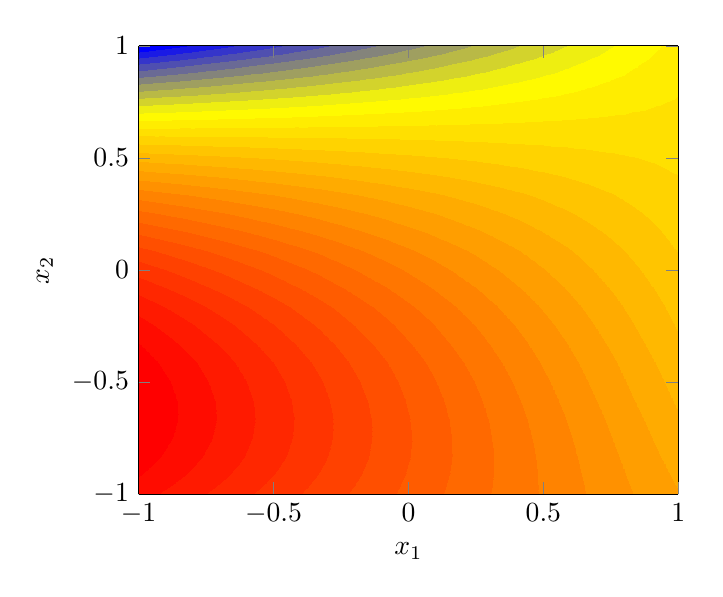
\begin{tikzpicture}[scale=1]
\begin{axis}[view={0}{90},
xlabel=$x_1$,ylabel=$x_2$]
\addplot3[contour filled={number = 30,labels={false}},domain=-1:1,y domain=-1:1] {y*(y-1)*(-x+1) + (y^2-1)*(2*x-1) + y*(1+y)*(x-2)};
\end{axis}
\end{tikzpicture}
\caption{Courbes de niveau de $f(x)$}
\end{subfigure}
\label{fig:exomni}
\caption{Exemple de mauvaise performance de la stratégie omnisciente}
\end{figure}

L'ordonnancement omniscient est impossible sans la connaissance au préalable de la valeur de la fonction objectif à chaque point de $P^k$.
La simulation du comportement de la stratégie peut être obtenue avec l'utilisation d'un ordonnancement en fonction d'un modèle, avec la fonction objectif elle-même comme modèle $\tilde{f}(x):=f(x)$. En terme d'évaluations de la fonction objectif, l'algorithme opportuniste avec ordonnancement omniscient aura le même coût que l'algorithme non-opportuniste. Cependant, la performance théorique de la stratégie omnisciente sera observable en considérant seulement $\frac{1}{|P^k|}$ pour chaque $k$ correspondant à une étape de \POLL fructueuse. Il est ainsi assuré que la stratégie omnisciente sera au moins aussi performante que la sonde complète. Cette performance serait en mesure de fournir une amélioration pour les autres stratégies. C'est d'autant plus vrai pour la stratégie d'ordonnancement à l'aide de modèles, dont les idées de base sont d'ordonnancer selon la meilleure diminution possible prédite par un modèle.
\subsection{Ordonnancement négatif-omniscient}\label{sec:neg}
Si l'opportunisme est susceptible d'influencer positivement la performance d'algorithmes d'optimisation, alors il a aussi le pouvoir de l'influencer négativement. Afin de pouvoir observer l'ampleur de l'impact négatif possible, il est possible d'identifier une stratégie d'ordonnancement qui fera exactement l'opposé de l'ordonnancement omniscient. On désignera cette stratégie d'ordonnancement comme \emph{l'ordonnancement négatif-omniscient}. Pour les itération de \POLL consistant en un succès, les points sont ordonnés de façon à forcer l'évaluation des points n'entrainant pas de succès en premier, pour ensuite évaluer le point entrainant l'amélioration la plus modeste possible.  
  
Encore une fois, il s'agit d'une stratégie avec aucune application pratique. Son unique utilité est de pouvoir simuler, selon notre intuition, l'obtention du pire ordre possible suivie d'une interruption prématurée de l'étape de \POLL. En pratique, il est possible d'obtenir ce comportement en utilisant ordonnancement en fonction d'un modèle, utilisant comme modèle une fonction retournant l'opposé de la fonction objectif $\tilde{f}(x):=-f(x)$. Il est difficile d'estimer le coût en terme d'évaluations de la fonction objectif, compte tenu que le nombre d'itération nécessaire à la convergence risque d'être plus élevé.  

Il est important de noter que la stratégie négatif-omnisciente n'est pas universellement la pire possible pour tout problème donné, au même titre que la stratégie omnisciente n'est pas la meilleure. Il s'agit de la pire dans l'optique où on veut minimiser le nombre d'évaluations de chaque étape de \POLL, sans considérer les impacts possibles sur les étapes de \SEARCH d'un algorithme.
\section{Mise en place de l'opportunisme}\label{sec:mis}
En forçant l'évaluation séquentielle de la fonction sur les candidats de $P^k$ et $S^k$, l'opportunisme demandent que les cadres algorithmiques soient plus restrictifs et limités à des formes séquentielles. L'application de la stratégie est limitée à certains algorithmes dont la forme permet son instauration. Les algorithmes de méthodes de régions de confiance~\cite{CoScVibook,CoGoTo00a} en optimisation sans-dérivées possèdent un seul candidat par itération de l'algorithme. D'autres ne peuvent être vus de façon non-opportuniste sans les dénaturer. Prenons, par exemple, les transformations géométriques générant les candidats à chaque étape d'une itération de Nelder Mead. Chacune de ces transformations pourrait être effectuée préalablement de façon à identifier l'ensemble des candidats possiblement rencontrés lors du déroulement d'une itération de l'algorithme, créant ainsi une liste de points à ordonnancer. Cependant, ceci mettrait en péril le bon fonctionnement de la méthode en détruisant les propriétés qui en font une méthode attrayante. Pour l'algorithme de Nelder Mead, si on considère une liste de points, on aura un ordonnancement sans aucune flexibilité.

La stratégie opportuniste est incompatible avec certains algorithmes, ce qui justifie la tâche d'identifier préalablement un ensemble d'algorithmes compatibles. Le critère de compatibilité principal consiste en l'existence d'une étape où une liste de points qui doit être évaluée, soient les étapes de \SEARCH et de \POLL ainsi que dans leurs équivalents dans \imfil. L'opportunisme ne doit pas modifier les hypothèses émises lors des analyses de convergence de ces algorithmes. Il est vérifié à la section 3.1 que c'est le cas pour les algorithmes étudiés dans le cadre de ce travail. La section qui suit détaille les modifications nécessaire à la mise en place de l'opportunisme dans les étapes de \POLL pour les algorithmes de recherche directe identifiés préalablement. 
  
La stratégie opportuniste réfère à l'arrêt prématuré des évaluations dans la sonde. Jusqu'ici, seulement la stratégie opportuniste la plus intuitive a été évoquée, soit celle de l'arrêt à l'obtention d'un premier succès. La définition de succès varie selon les algorithmes, et diverses stratégies opportunistes peuvent être élaborées sur mesure en fonction de l'étape de \POLL de la méthode à l'étude. Dans cette section, on définit les différentes versions de l'opportunisme applicables aux étapes de \POLL de \CS, \GPS, \GSS et \MADS et dont la performance est étudiée.  
  
\begin{definition}[Stratégie opportuniste au $p$\textsuperscript{ème} succès]
\label{def:oppemesucces}
La stratégie opportuniste au p\textsuperscript{ème} succès désigne l'arrêt prématuré de l'étape de \SEARCH ou de \POLL courante d'un algorithme de recherche directe après l'obtention de $p$ points satisfaisants le critère de succès de l'algorithme, soit la diminution simple ou la diminution suffisante.
\end{definition}
La stratégie opportuniste au $p$\textsuperscript{ème} succès consiste à attendre l'évaluation de $p$ points de sonde qui satisfont le critère de succès avant de procéder à la prochaine itération de l'algorithme avec le meilleur candidat évalué comme nouvel itéré courant $x^k$ . Cette variation est destinée à modérer l'utilisation de la stratégie opportuniste simple et à la rendre plus robuste. Par exemple, un point de sonde entrainant une diminution minime, par exemple le fruit d'un bruit stochastique présent dans la boîte noire, pourrait être considéré à tort comme un nouveau succès par un algorithme opportuniste.   
  
L'opportunisme au $p$\textsuperscript{ème} succès propose de décaler l'arrêt de la sonde. Ce décalage dépend du nombre points entrainant un succès identifiés en cours de celle-ci. Il est possible d'utiliser d'autres mécaniques pour prolonger la sonde tout en étant opportuniste.

\begin{definition}[Stratégie opportuniste avec un minimum de $q$ évaluations]
	\label{def:opmineval}
	La stratégie opportuniste minimum $q$ évaluations désigne l'arrête prématuré de l'étape de \SEARCH ou de \POLL courante d'un algorithme de recherche directe après $q$ évaluations si un point $\tau$ satisfaisant le critère de succès de l'algorithme est évalué au cours des $q$ premières évaluations. Dans le cas contraire, l'arrêt prématuré se fait à la première obtention d'un point $\tau$ satisfaisant le critère de succès de l'algorithme
\end{definition}

La stratégie opportuniste avec un minimum de $q$ évaluations est une autre déclinaison de l'opportunisme. Elle permet un autre type de contrôle sur le décalage de l'interruption de la sonde qui peut être utile selon la méthode utilisée. Par exemple, une étape de \SEARCH dont le fonctionnement dépends de l'évaluation d'un ensemble de points bien dispersés pourrait bénéficier d'une sonde avec un minimum d'évaluations, sans nécéssité que plus d'un des points entraine un succès. 

Les différentes stratégies opportunistes sont applicables aux étapes de \POLL des algorithmes de recherche suivant l'algorithme \ref{alg:oppPoll}.
\begin{algorithm}[H]
	\caption{\textsf{\POLL opportuniste}}
	\label{alg:oppPoll}
	\begin{algorithmic}
		\STATE Avec $f:\R^n \mapsto \R$ la fonction objectif et $x^0$ le point de départ
		\STATE 1. \POLL
		\bindent
		\STATE Ordonner $P^k$ avec la stratégie d'ordonnancement choisie.
		\FOR { $t \in P^k$}
		\IF {Critère d'arrêt opportuniste de la sonde}
		\STATE $x^{k+1} \in \arg \min \{f(t) : t \in P^k_e\}t$ avec $P^k_e$ les points de l'ensemble de sonde qui ont été évalués.
		\STATE Mise à jour de $\delta^k$ et $\Delta^k$ selon un succès de l'étape
		\STATE Fin de la sonde, poursuivre à la terminaison.
		\ENDIF
		\STATE $x^{k+1} \leftarrow x^{k}$
		\STATE Mise à jour de $\delta^k$ et $\Delta^k$ selon un échec de l'étape
		\ENDFOR
		\STATE Fin de la sonde, poursuivre à la terminaison.
		\eindent
	\end{algorithmic}
\end{algorithm}
Ce cadre algorithmique n'est pas applicable à la cinquième méthode présentée, soit \imfil. Dans son œuvre élaborant les principes de sa méthode~\cite{Kelley2011}, Kelley commente la relation de \imfil à l'opportunisme.
\begin{quote}
	<<La version opportuniste de \CS est de plusieurs façons plus naturelle que la version non-opportuniste (pensez à un animal cherchant de la nourriture). Toutefois, \imfil est une méthode conceptuellement non-opportuniste. La raison de ce choix est que \imfil utilise un échantillonnage pour approximer un gradient et donc une direction de recherche et pour construire un modèle de $f$.>>
\end{quote}
L'utilisation de l'opportunisme dans \imfil nécessite une adaptation partielle de la méthode. Premièrement, la notion de succès pour \imfil est différente de celle établie pour les autres algorithmes identifiés. On dira que la sonde du stencil comporte un succès si il existe un point $t$ dans $P^k := \{x^k+h^kv_i: v_i \in V\}$ pour lequel $f(t)<f(x^k)$. Pour respecter la définition \ref{def:ordo} de l'opportunisme sans compromis, on devrait terminer la sonde du stencil au premier succès. On désignera cette méthode comme \textsf{\imfil-op} pour \imfil avec opportunisme pur. \imfil enchaîne l'étape de sonde du stencil avec une descente du gradient. C'est cette dernière qui confère un intérêt à la méthode, d'autant plus que la qualité de sa contribution est dépendante du nombre de points calculés dans la sonde du stencil. L'interruption prématurée de la sonde du stencil empêchera l'obtention de l'information nécessaire pour la détermination d'une direction de descente cohérente, puisque celle-ci est déterminée à l'aide de différences finies obtenues avec les valeurs de la fonction objectif aux points de $P^k$. Prenons pour exemple l'obtention d'un succès à une première évaluation dans la sonde. En ayant échantillonné seulement dans un sous-espace de dimension 1, dans un espace de dimension $n$, le gradient du stencil aura $n-1$ composantes nulles. On anticipe alors que cette stratégie nuira au bon fonctionnement pratique de la méthode.
\begin{algorithm}[H]
 	\caption{\textsf{Sonde du stencil \imfil-op}}
 	\label{alg:imfilop}
 	\begin{algorithmic}
 		\STATE Avec $f:\R^n \rightarrow \R$ la fonction objectif et $x^0$ le point de départ
 		\STATE Poser $P^k := \{x^k+h^kv_i: v_i \in V\}$ et ordonner selon la stratégie d'ordonnancement choisie.
 		\FOR {$t \in P^k$}
 		\IF {$f(t) < f(x^{k+1})$}
 		\STATE $x^{k+1} \leftarrow t$
 		\STATE Fin de la sonde, poursuivre à la recherche linéaire
 		\ENDIF
 		\ENDFOR
 		\STATE Fin de la sonde, poursuivre à la recherche linéaire
 	 	\end{algorithmic}
\end{algorithm}
Pour éviter les cas avec des directions comportant plusieurs composantes nulles, on propose une autre version de l'algorithme incorporant la stratégie opportuniste. Rappelons que pour \imfil est une algorithme d'optimisation sous contraintes de bornes. Il utilise le motif $V = \{\pm e_i : i=1,\dots,n\}$ formé par les directions élémentaires, duquel découle un gradient du stencil $\nabla_{s}f(x^k) = \frac{1}{h^k}\delta(f,x^k,V,h)V^{\dagger}$. En considérant le cas le plus restrictif en terme de points réalisables, $x^k$ se trouve à la frontière de $n$ contraintes actives. Les $n$ points du motif, maintenant superposés à $x^k$, figurant dans $\Omega$ seront nécessaires pour évaluer $n$ différences finies avant, qui fourniront une approximation du gradient dans chaque dimension de $n$. Ces approximations sont moins précises tel que le stipule le théorème de Taylor, soit $O(h)$ plutôt que $O(h^2)$ dans le cas de \imfil sans opportunisme, où chaque approximation est calculée avec une différence centrée.   
  
L'idée de la deuxième approche est de favoriser l'utilisation de différences avant dans le calcul de $\nabla_{s}f(x^k)$, à l'instar du cas précédemment décrit. Le fonctionnement de l'algorithme serait le suivant. En premier lieu, les points $x^k+h^ke_j$ et $x^k-h^ke_j$ sont ordonnés deux à deux avec la stratégie d'ordonnancement choisie. Dans le cas où une contrainte est active pour la dimension $j$ tel que $x^k+h^ke_j \notin \Omega$ ou $x^k-h^ke_j \notin \Omega$, aucun ordonnancement est nécessaire pour cette paire et c'est le point réalisable qui est considéré comme le premier. Ensuite, on évalue $f$ pour les $n$ premiers points des $W_j$ définis à l'étape précédente. Si un succès est encouru, alors la sonde du stencil s'arrête et on procède à la recherche linéaire. Si aucun point n'a entrainé de diminution simple, alors on ré-ordonne les points restants, soient les deuxièmes points dans les paires, avec la même stratégie choisie et on poursuit la sonde du stencil de façon opportuniste.  
  
La méthode proposée implique au minimum une approximation du gradient dans chaque dimension et incorpore la notion d'opportunisme. Pour chaque étape de sonde, $n$ évaluations peuvent être sauvées. Cependant, pour chaque étape de sonde fructueuse dont la recherche linéaire subséquente est non-fructueuse, les évaluations supplémentaires auront été en vain. On désignera cette méthode comme \textsf{\imfil-od} pour \imfil avec opportunisme dimensionnel. Le cadre algorithmique présenté est généralisé pour le cas où tous les points du motif $V$ sont réalisables. Les ensembles $W_i$ y représentent les ensembles de deux points opposés dans $V$.
\begin{algorithm}[H]
	\caption{\textsf{Sonde du stencil \imfil-od}}
	\label{alg:imfil-od}
	\begin{algorithmic}
		\STATE Avec $f:\R^n \mapsto \R$ la fonction objectif et $x^0$ le point de départ
		\STATE 
			Soit la paire de points $x^k+h^k v_i$ et $x^k-h^k v_i$. Ordonner selon la stratégie d'ordonnancement choisie pour tout $i$. Poser $W_{i,1}$ le point apparaissant en premier dans l'ensemble et $W_{i,2}$ le point apparaissant en deuxième.	 
		\STATE Poser $P^k_1 := \{W_{i,1}~:~i=1,2,\dots,n\}$
		\STATE $x^{k+1} \in \arg\min\{f(x) : x \in P^k_1 \cup \{x^k\}\}$
		\IF {$x^{k+1}\neq x^k$}
		\STATE Fin de la sonde, poursuivre à la recherche linéaire
		\ENDIF
		\STATE Poser $P^k_2 := \{W_{i,2}~:~i=1,2,\dots,n\}$ et ordonner $P^k_2$ selon la stratégie d'ordonnancement choisie
		\FOR {$t \in P^k_2$}
		\IF {$f(t) < f(x^{k+1})$}
		\STATE $x^{k+1} \leftarrow t$
		\STATE Fin de la sonde, poursuivre à la recherche linéaire
		\ENDIF
		\ENDFOR
		\STATE Fin de la sonde, poursuivre à la recherche linéaire
	\end{algorithmic}
\end{algorithm}  